% Setup - do not change
\documentclass[11pt]{article}
\usepackage[top=0.9in, left=0.9in, bottom=0.9in, right=0.9in]{geometry} 
\usepackage{parskip}

\usepackage[english]{babel}
\usepackage[utf8]{inputenc}
\usepackage{amsmath,amsthm,amssymb,graphicx,pdfpages,lipsum,hyperref}
\usepackage[none]{hyphenat}
\usepackage{csquotes}
\setlength\parindent{0pt}
%%%%%%%%%%%%%%%%%%%%%%%%%%%%%%%%%%%%%%%%%%%%%%%%%%%%%%%%%%%%%%%%%%%
% add other packages here if required

%% Bibliography are specified in this file. You can also choose inline bib style if you want to. But make sure your citation style is consistent (and proper)
% For more details on citation: https://library.unimelb.edu.au/recite
\usepackage[sorting = none]{biblatex}
\addbibresource{references.bib}

%%%%%%%%%%%%%%%%%%%%%%%%%%%%%%%%%%%%%%%%%%%%%%%%%%%%%%%%%%%%%%%%%%% the '%' symbol denotes comments

% Begin document creation
% DELETE THE \lipsum PLACEHOLDERS WHEN YOU BEGIN
\title{\textbf{Analyzing the Impact of Weather and Urban Dynamics on Yellow Taxi NYC}}
\author{
Yicong Yao \\
Student ID: 1302642 \\
%% Replace the link with your github repo
% 1. Remember to escape underscore (\_) in the link.
% 2. Remember to include the commit you want to submit in the link
\href{https://github.com/MAST30034-AppliedDataScience/project-1-individual-YicongYao.git}{Github repo with commit}
}

\begin{document}
\maketitle

\section{Introduction}


In the bustling streets of New York City, Yellow Taxis not only paint the town with their iconic color but also serve as a critical mode of transportation for millions. This project delves into the factors influencing the economics of these taxi services, particularly focusing on how various weather conditions impact taxi operations. Our analysis is anchored on data spanning from December 2023 to May 2024, a period that presents a rich tapestry of weather variations from winter's chill to spring's warmth.

We chose the Yellow Taxi trip records \cite{NYCdata} for this study because of their comprehensive availability and the robustness of the dataset which includes detailed trip attributes such as distance, duration, and fares, alongside we use external weahter data \cite{Weatherdata}, which contains environmental conditions like temperature and precipitation. This choice allows for a nuanced exploration of the interplay between weather and taxi travel patterns, providing insights that could benefit a wide range of stakeholders from policy makers to daily commuters.

To enrich our analysis, external weather datasets were integrated, offering precise daily weather conditions. This combination not only strengthens the study's foundational data but also enhances the reliability of our findings by correlating taxi trip metrics with specific weather events. All data used in this analysis, including sources and collection methods, is fully documented and accessible, ensuring transparency and reproducibility of the research.

The methodology of this project employs a dual approach: descriptive statistics to outline general trends and machine learning models to quantify the impact of weather on fare amounts. By employing Linear Regression and Random Forest models, we aim to not only predict fare amounts under different weather conditions but also understand which factors most significantly affect those predictions. This layered approach provides both a broad and detailed view of the dynamics at play, equipping stakeholders with the knowledge to make informed decisions. \cite{nyctaxi2016}

In essence, this project not only seeks to highlight patterns and anomalies within the Yellow Taxi operations but also to offer actionable recommendations based on quantitative analysis, thereby contributing to the efficient management of urban transportation in varying weather conditions.

\section{Preprocessing}
Before diving into our analysis, we needed to clean up and organize our data. This process, called preprocessing, is super important because it helps us make sure our results are accurate and meaningful. We worked with two main datasets: the Yellow Taxi Trip Records and some weather data we got from an external source. Let's break down what we did for each.

For the Yellow Taxi Trip Records, we started by simplifying things. We removed a bunch of columns we didn't need, like 'store\_and\_fwd\_flag', 'Airport\_fee', and 'VendorID'. These columns didn't really help us understand taxi usage patterns, so we got rid of them to make our dataset easier to work with. Next, we had to deal with missing information. For example, sometimes the 'passenger\_count' was missing. We decided to fill these gaps with 0, assuming that if no one recorded the number of passengers, it probably meant there weren't any. This might not be perfect, but it's a reasonable guess based on how the data is usually entered.

We also had to clean up some weird data entries. Sometimes, the data would show impossible things, like trips with more than 4 passengers (taxis usually can't fit that many people) or trips longer than 50 miles (which is pretty rare for city taxis). We removed these unusual entries to focus on typical taxi rides. This helps us avoid having these odd cases mess up our analysis. After cleaning, we created some new useful information. For instance, we calculated how long each trip took and noted what hour of the day the trip started. This new info helps us look for patterns in when people use taxis and how long their trips usually are.


For the weather data, we kept things focused on what we thought might affect taxi rides. We kept information like temperature and whether it was raining, but got rid of less relevant stuff like sunrise and sunset times. The cool part was combining this weather data with our taxi data. We matched up the weather conditions with each taxi ride based on when the ride happened. This way, we could see if rainy days meant more taxi rides, or if super hot days changed how people used taxis.



After all this cleaning and combining, we ended up with a massive dataset of over 13 million taxi rides, each with its own weather information. This is a lot of data to work with! It gives us a really good foundation for our analysis. With this preprocessed data, we can start looking for interesting patterns. For example, we might be able to see how rain affects the number of taxi rides, or if people take longer trips when it's cold out. By carefully preparing our data like this, we've set ourselves up to discover some really interesting things about how taxis are used in the city and how weather might play a role in that.




\section{Analysis and Geospatial Visualisation}
Our comprehensive analysis utilizes temporal and geospatial data alongside fare and weather impact assessments to uncover patterns that influence taxi operations in New York City.

\subsection{Temporal Analysis}
From the temporal analysis (Figure\ref{fig:1}), it is evident that there are distinct peaks and troughs in the number of trips throughout the day. The highest number of trips consistently occurs during evening rush hours, suggesting that commuters heavily rely on taxis for returning home. Additionally, there's a noticeable dip in the early hours, which corresponds to the least active period for taxis. This information is crucial for dispatch planning and for drivers to maximize their daily earnings by targeting peak hours.

\begin{figure}[h]
    % change the scale multiplier to make the figures smaller or larger
    \includegraphics[width=.85\textwidth]{image/Temporal Analysis.png}
    % this ensures your figures are centered where possible
    \centering
    \caption{Temporal Analysis} % refer to this image as (Figure 1)
    \label{fig:1}
    
\end{figure}



\subsection{Geospatial Analysis}
The geospatial analysis (Figure\ref{fig:2}) provides insights into the average passenger count and total amount collected across different drop-off locations. Areas such as airports and major commercial districts show higher average fares and passenger counts, underscoring their importance in overall taxi revenue. This highlights potential high-demand areas where taxi operators could focus their services.\cite{urbanmobility2018}

\begin{figure}[h]
    % change the scale multiplier to make the figures smaller or larger
    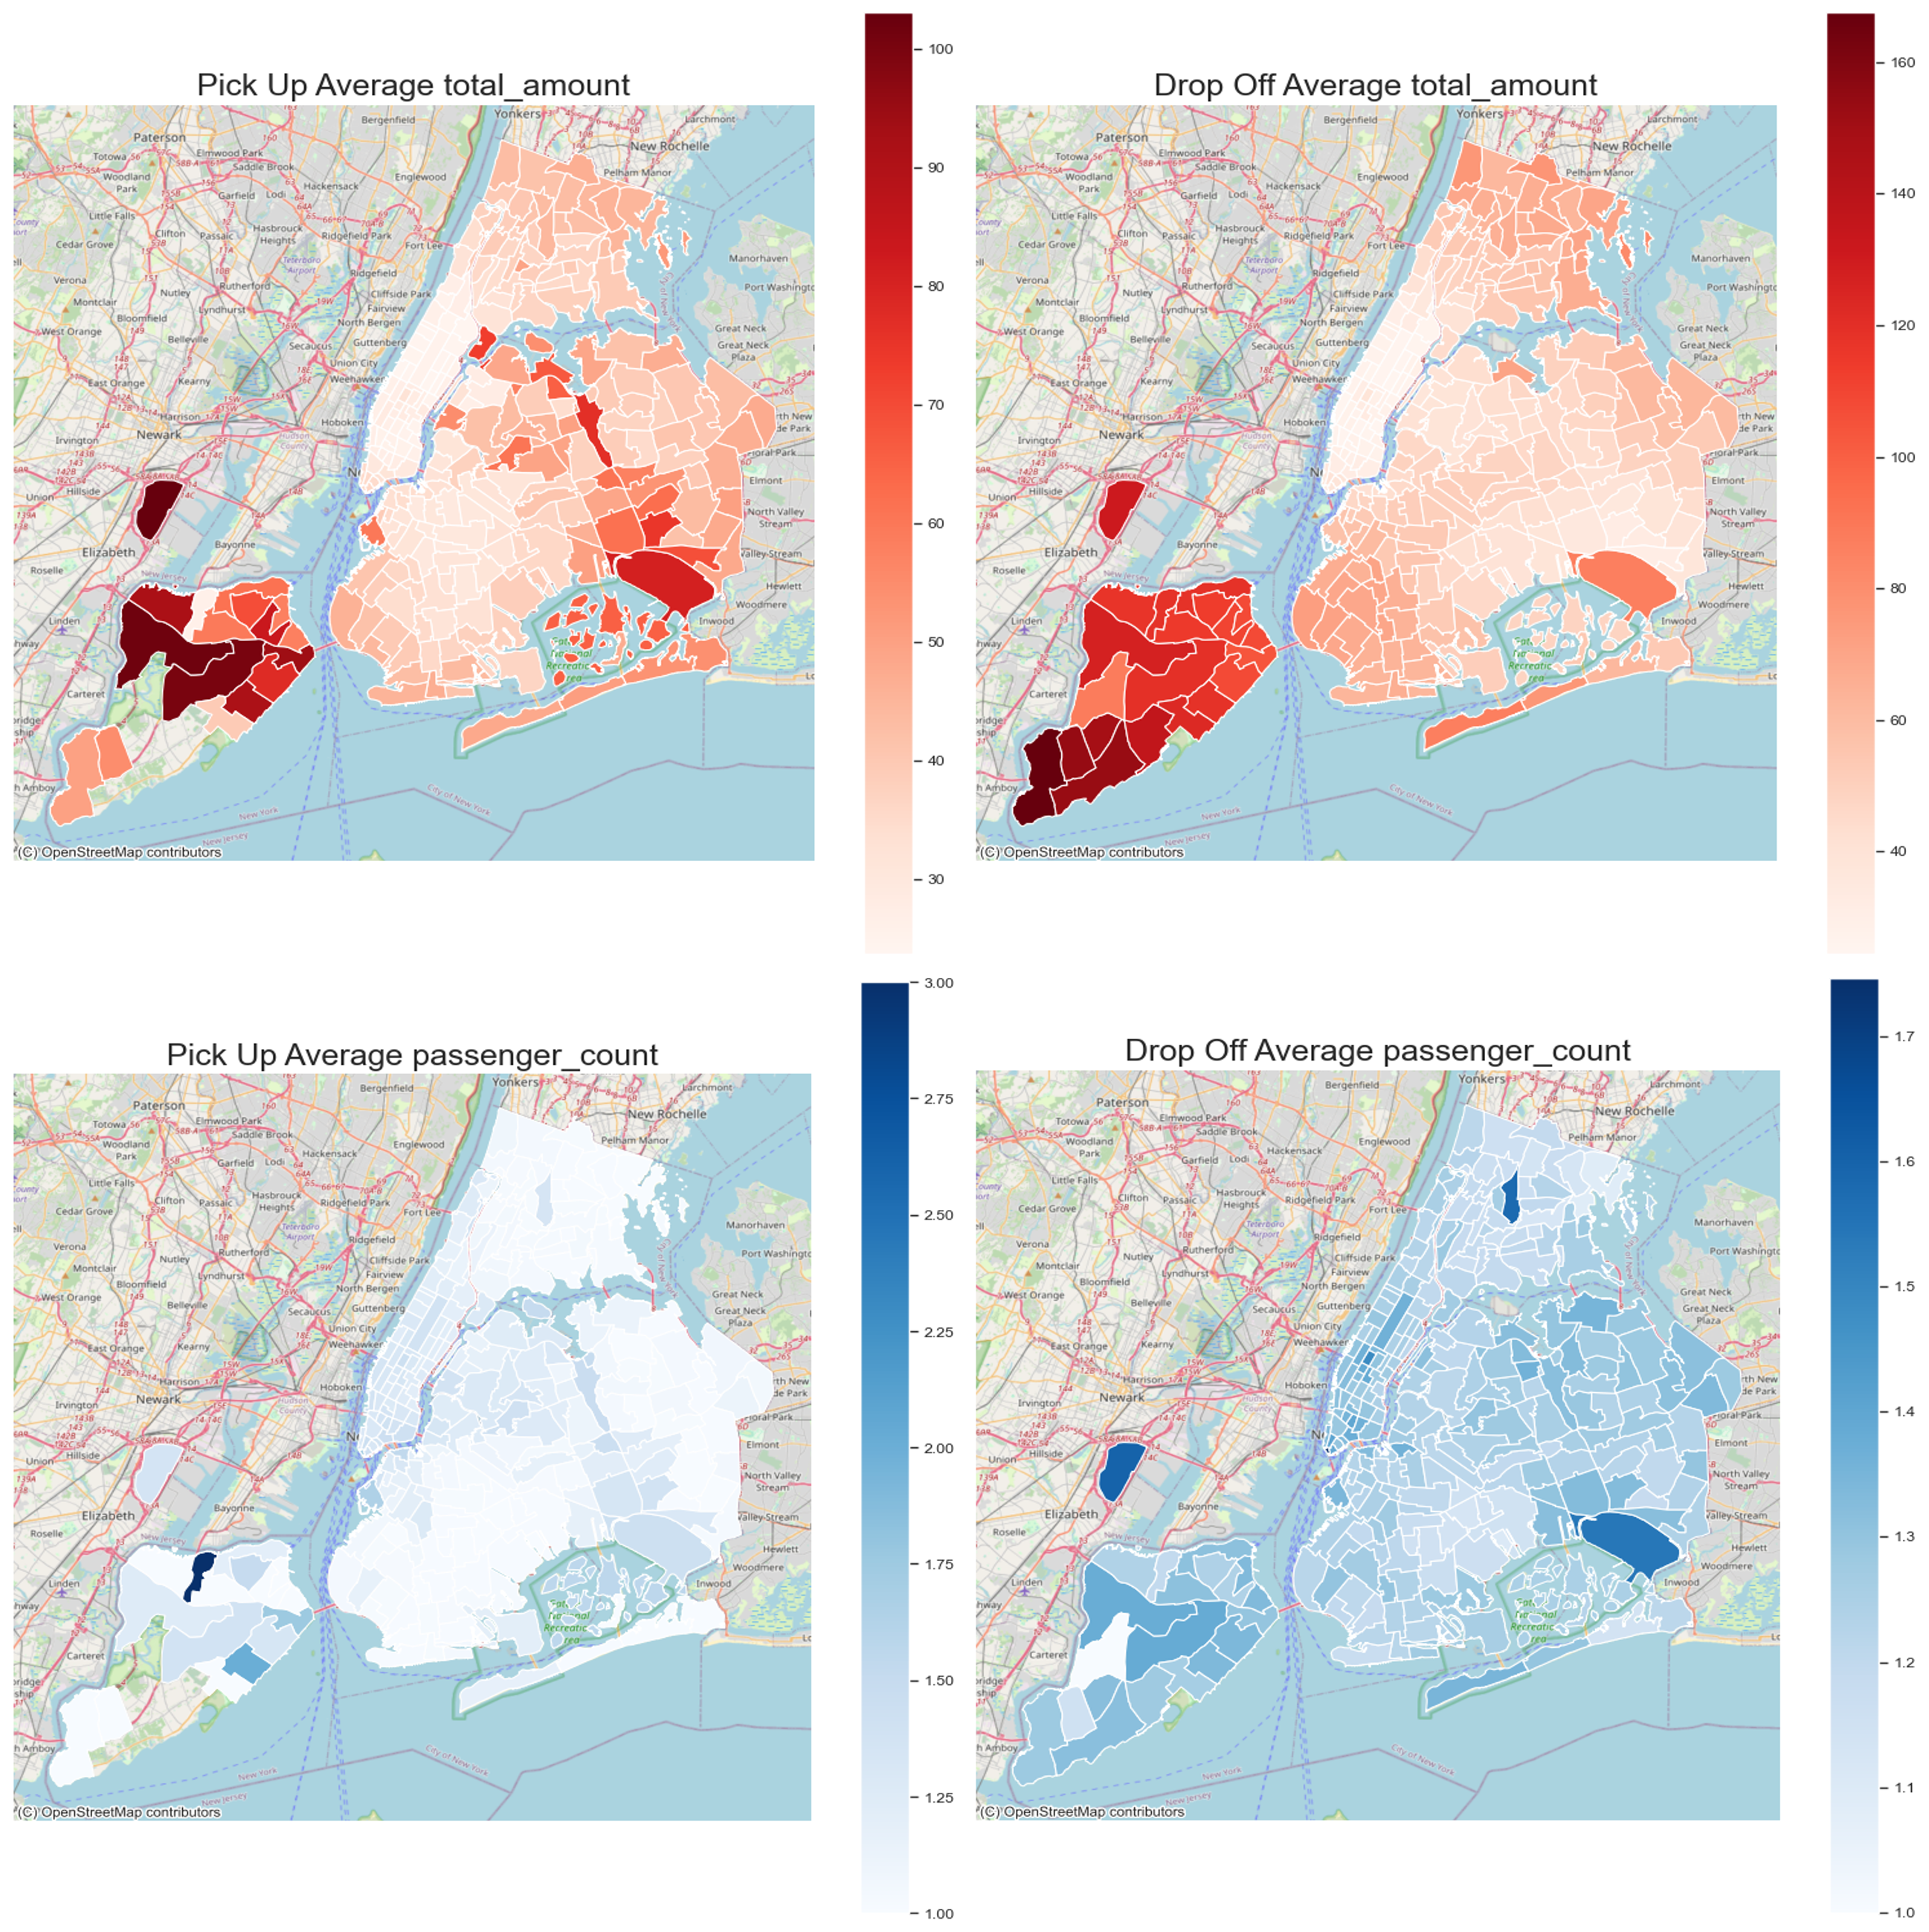
\includegraphics[width=.85\textwidth]{image/geo.png}
    % this ensures your figures are centered where possible
    \centering
    \caption{Geospatial Analysis} % refer to this image as (Figure 1)
    \label{fig:2}
    
\end{figure}


\subsection{Fare Analysis}
In the fare analysis (Figure \ref{fig:3}), we observed a wide range of fare amounts, with most trips costing between \$10 and \$25. The distribution is right-skewed, indicating that while most trips are relatively short and inexpensive, there are occasional longer trips that significantly increase the fare amount. Understanding this distribution helps in setting realistic expectations for drivers about potential earnings and in strategizing for longer routes. 

\begin{figure}[h]
    % change the scale multiplier to make the figures smaller or larger
    \includegraphics[width=.85\textwidth]{image/fare.png}
    % this ensures your figures are centered where possible
    \centering
    \caption{Fare Analysis} % refer to this image as (Figure 1)
    \label{fig:3}
    
\end{figure}

\subsection{Weather Impact Analysis}
The weather impact analysis (Figure \ref{fig:4}) shows how different weather conditions affect taxi usage. For example, rainy and snowy days see an increase in trip distances and fares, possibly due to reduced availability of other forms of transport and the higher inconvenience of walking. This suggests that taxis are a preferred mode of transport during adverse weather conditions, which could be used by taxi companies to adjust fares or increase fleet availability in anticipation of bad weather. \cite{weatherimpact2020}

\begin{figure}[h]
    % change the scale multiplier to make the figures smaller or larger
    \includegraphics[width=1\textwidth]{image/weather.png}
    % this ensures your figures are centered where possible
    \centering
    \caption{Weather Impact Analysis} % refer to this image as (Figure 1)
    \label{fig:4}
    
\end{figure}


\begin{figure}[h]
    % change the scale multiplier to make the figures smaller or larger
    \includegraphics[width=.55\textwidth]{image/Weather Impact heatmap.png}
    % this ensures your figures are centered where possible
    \centering
    \caption{Weather Impact Analysis Heatmap} % refer to this image as (Figure 1)
    \label{fig:5}
    
\end{figure}

\subsection{Weather Effect on Tips}
Finally, our analysis of tipping patterns in relation to weather conditions (Figure \ref{fig:6}) reveals that tips tend to be higher on clear days and lower during adverse weather conditions such as snow. This could be attributed to the quicker trips and better overall mood of passengers on clearer days, while the stress and longer travel times during bad weather might reduce the propensity to tip.

\begin{figure}[h]
    % change the scale multiplier to make the figures smaller or larger
    \includegraphics[width=.45\textwidth]{image/Weather Impact tip.png}
    % this ensures your figures are centered where possible
    \centering
    \caption{Weather Effect on Tips} % refer to this image as (Figure 1)
    \label{fig:6}
    
\end{figure}

Each of these analyses provides actionable insights for taxi operators. By understanding temporal and spatial patterns, as well as the impact of weather on taxi usage and revenue, operators can optimize their strategies to enhance service availability and profitability. Moreover, these findings could be useful for urban planners in understanding mobility patterns in the city, facilitating better infrastructure development and public transport scheduling to complement taxi services.



\section{Modelling}
To further our understanding of how various factors affect taxi fares in New York City, we employed two different statistical models: Linear Regression and Random Forest Regression. These models were chosen to analyze the relationships between multiple variables (like weather conditions, trip distances, and time features) and the total fare amount, which is our primary target variable.

\subsection{Model Specification and Justification}
Linear Regression is used because of its efficiency in determining the linear relationship between independent variables and the dependent variable. It's particularly useful for interpreting the direct effect of predictors on the outcome, providing clear insights into how each factor such as temperature or precipitation affects fare amounts. Random Forest Regression was selected for its robustness in handling non-linear data and its ability to manage overfitting. This model is effective in capturing complex patterns from data, which might be missed by simpler models like Linear Regression.\cite{datadriven2017}


\subsection{Assumptions and Model Suitability}
We assume that features like trip distance and weather conditions have a linear or non-linear relationship with the fare amount. The Linear Regression model treats all independent variables as continuous, while the Random Forest model can inherently handle the non-linearity among them.
Continuous variables used in our models include 'trip\_distance', 'temp', 'humidity', and 'wind speed'. We carefully ensured that the usage of these features aligns with the capabilities of our chosen models to prevent inappropriate application and potential bias.

\subsection{Model Performance and Analysis}
Both models were trained on a subset of the data from December 2023 to May 2024 and were tested using separate data to ensure that predictions reflect future conditions accurately. The models' performances were evaluated using standard metrics like Mean Absolute Error (MAE), Mean Squared Error (MSE), and R-squared, which are summarized in the table:

\begin{table}[]
\centering
\begin{tabular}{|l|l|l|l|}
\hline
Model             & \multicolumn{1}{c|}{MAE} & \multicolumn{1}{c|}{MSE} & \multicolumn{1}{c|}{R-squared} \\ \hline
Linear Regression & 4.883365                    & 60.806086                & 0.877288                     \\ \hline
Random Forest     & 4.943383                    & 62.942562                & 0.872976                        \\ \hline
\end{tabular}
\end{table}

\subsection{Feature Importance and Model Insights}
The Random Forest model provided a detailed view of feature importance, indicating that 'trip\_distance' and 'weather conditions' are significant predictors of fare amounts (as shown in the Figure \ref{fig:7}). This suggests that longer trips and severe weather significantly increase fares. Linear Regression coefficients (shown in the Linear Regression Coefficients Figure \ref{fig:7}) also highlighted that trip distance has the most substantial positive impact on fare, while some weather conditions like heavy precipitation slightly decrease the fare amount, possibly due to fewer people choosing to travel.The findings from our models suggest specific strategies for taxi drivers. For instance, targeting longer trips and working during adverse weather conditions could potentially increase earnings. These models can also aid fleet operators in strategic planning and operational adjustments based on predicted fare amounts under different conditions.

\begin{figure}[h]
    % change the scale multiplier to make the figures smaller or larger
    \includegraphics[width=1.\textwidth]{image/model.png}
    % this ensures your figures are centered where possible
    \centering
    \caption{Feature Importance} % refer to this image as (Figure 1)
    \label{fig:7}
    
\end{figure}

\section{Discussion}
Our analysis of New York City's taxi operations reveals some interesting patterns. We found that weather plays a big role in how taxis operate. On rainy or snowy days, people tend to take longer trips and pay more. This makes sense - who wants to walk in the rain, right? We also noticed that certain times are busier for taxis, like during evening rush hour and on weekends. If you're a taxi driver, you might want to work more during these times to make more money.

We also looked at where people take taxis most often. Unsurprisingly, airports and busy business areas are popular spots. Drivers could focus on these areas to get more passengers. Lastly, we found that people tend to tip more on nice, clear days. Maybe it's because their trips are shorter, or maybe they're just in a better mood when the sun is shining. All of these findings could help taxi drivers and companies make smarter decisions about when and where to work.

\section{Recommendations}
Based on what we found in our study, we have a couple of suggestions for taxi companies in New York City. First, it might be a good idea for taxi drivers to work more when the weather is bad, like during rainy or snowy days. We noticed that people take longer trips and pay more during these times. Also, evening rush hours are super busy, so drivers could make more money if they work then.
Another tip is to focus on busy areas like airports and business districts. These places always have lots of people looking for taxis. If drivers hang out near these spots, they'll probably get more passengers and make more money. To make all this work, taxi companies might need to use some fancy tech to keep track of the weather and where people need rides. They could also maybe give bonuses to drivers who work during the not-so-fun times, like in bad weather or late at night. This way, there will always be taxis available when people need them most.

\section{Conclusion}
Our analysis of New York City's Yellow Taxi services demonstrates a significant influence of weather conditions, time, and geographical factors on taxi operations. Adverse weather increases trip distances and fares, while peak demand during evening hours and specific locations like airports and business districts offer potential for increased earnings. Based on these insights, we recommend optimizing driver schedules to align with peak demand and strategically deploying taxis to high-demand areas to maximize profitability.

Implementing these data-driven strategies can enhance the operational efficiency of taxi services, providing a model for effective urban transportation management that can be adapted to other cities. This project highlights the value of integrating diverse datasets to uncover actionable insights, paving the way for smarter, more efficient urban mobility solutions.



\clearpage

% BEGIN REFERENCES SECTION
\printbibliography

\end{document}